\chapter{Modelling exposure}
\label{chap:exposure}

Whilst we started our focus on modelling exposure and claims by firstly looking at the claims generators in chapter \ref{chap:claims} (this makes sense, as in the real world, claims occur even without being exposed to insurance contracts), we will now learn how to model the exposure of an insurance company by use of a simple two-level hierarchy. The first level of the hierarchy consists of \term{Underwriting Segments} and the second of \term{Lines of Business}. The former consists of the lowest available level of underwriting information, such as \textit{motor hull} or \textit{motor tpl}; the latter either consists of one line of business only or of a group of lines of business: \textit{motor} $=$ \textit{motor hull} $\cup$ \textit{motor tpl}. Depending on the granularity of the available data, underwriting segments might be granular to any level you can dream of: type of business, currency, region, legal entity, etc.~It is your professional judgement on the data available on which level you want to run simulations. Modelling every single contract will most often be too granular, modelling the whole company only will most often be too general.\footnote{Both extremes are existing in the real life: A reinsurer covering a niche might model contract by contract; a relatively small legal entitiy within a relatively large group will be modelled as one underwriting segment.}

\begin{figure}[htb]
	\centering
		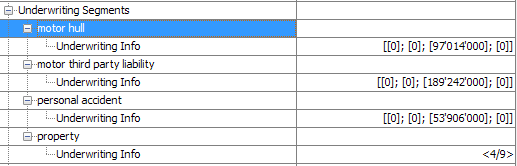
\includegraphics[scale=0.6]{images/UnderwritingSegments.png}
	\caption{Underwriting Segments}
	\label{fig:UnderwritingSegments}
\end{figure}

\begin{figure}[htb]
	\centering
		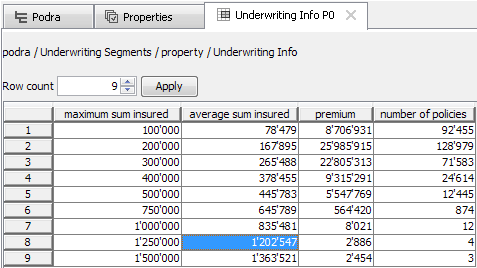
\includegraphics[scale=0.6]{images/UnderwritingSegmentsProperty.png}
	\caption{Underwriting Segments: Details for Property shown in a 4/9 matrix above}
	\label{fig:UnderwritingSegmentsProperty}  
\end{figure}


\begin{figure}[htb]
	\centering
		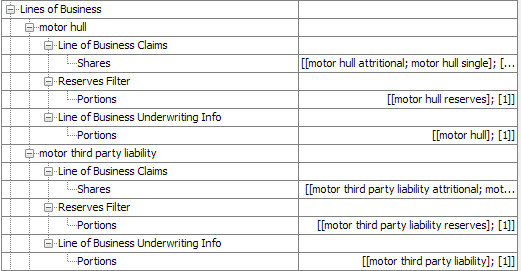
\includegraphics[scale=0.6]{images/LOB.png}
	\caption{Lines of Business}
	\label{fig:LOB}
\end{figure}

\section{Underwriting Segments}
\label{sec:underwritingsegments}
For the sake of convenience, a new underwriting segment can either be built by right-clicking on \term{Underwriting Segment} and selecting \term{add} -- resulting in an empty underwriting segment -- or by right-clicking an existing segment and selecting \term{duplicate}: The latter will copy all information from the `parent' underwriting segment to the `child' being saved under a new name.

The underwriting information contains per segment: \textit{maximum sum insured}, \textit{average sum insured}, \textit{premium} and \textit{number of policies}. It is possible and often appropriate to edit serveral risk bands: These risk bands will be used for surplus share treaty reinsurance (\cf Section~\ref{sec:ProportionalReinsurance}). It is important to remember these risk bands are directly interlinked to each other as shown in the following table:


\begin{table}[h]
\centering
\begin{tabular}{|l|l|l|}
\hline
Risk band $r_i$ & Minimum Sum Insured & Maximum Sum Insured \\
$r_1$ & $0$ & max$_1$ $=$ User Input \\
$r_2$ & max$_1$ & max$_2$ $=$ User Input \\
$r_3$ & max$_2$ & max$_3$ $=$ User Input \\
\ldots & \ldots & \ldots \\ 
\hline
\end{tabular}
	\caption{Risk Bands}
	\label{tab:RiskBands}
\end{table}


\note{Therefore, it is not possible to `group' a heterogenious portfolio after the merger of two companies, even if one of them with higher insured amounts, the other with lower insured amounts etc. This would rather be achieved by building a Line of Business as explained in the next section.} 

Double-clicking on the cell next to \term{Underwriting Info} opens a table where you select the number of bands needed and type in the criteria for each band:

\begin{itemize}
	\item \term{maximum sum insured}: The upper bound of the range of sums insured. The lower bound is given by the upper bound of the previous
class (in the previous row) or 0, \cf Table~\ref{tab:RiskBands}.
	\item \term{average sum insured}: The average sum insured of the policies included in the given risk class. By definition, the average should be
smaller than or equal to the maximum sum insured of the given row, but larger than the maximum sum insured of the previous row.
\item \term{premium}: The total premium of all the policies included in the risk band.
\item \term{number of policies}: The number of policies included in the risk band.

\end{itemize}

Note that the risk bands have to be in ascending order.

\section{Lines of Business}

Lines of business are built by the union of one or several underwriting segments; exposing them to claims generators and reserve filters. 

As now the risks are defined they may be combined or allocated to business segments. Adding a new line of business (right-click, as usual) opens three sets of parameters: Adding different claims generators (or shares\footnote{The share might be greater than $1$ in case you want to scale the distribution.} of them) to the dedicated Line of Business, as well as Reserve Filters (\cf~Section~\ref{sec:ReserveGenerators}). Finally, to each Line of Business the Underwriting Information is attached, completing the information needed in this area.

\todo{If you want to further cascade the grouping, \ie~looking at \term{Non Life} business consisting of motor and fire, sticking with the above example, you have to setup a line of business on the level of the existing granular underwriting segments: \textit{Non Life} $=$ \textit{motor hull} $\cup$ \textit{motor tpl} $\cup$ \textit{fire}. This allows separate modelling of company-wide effects such as inflation for underwriting segments in specific countries.}{Is this true?}
